\section{Aspetti implementativi}



\subsection{Il desing pattern MVC}

\subsection{Implementazione dello schema di gioco}

\begin{figure}
\includegraphics[scale=0.4]{img/modelClassDiagram.png}
\end{figure}

\subsection{L'interfaccia grafica}
\subsection{La gestione e la distribuzione della rete}
	\subsubsection{Registrazione presso la lobby}
		Il primo passo svolto da ogni nodo di rete e' la registrazione
		presso un server centralizzato comune, implementante diverse
		"stanze" di gioco; le cosiddette lobby.\\
		Questo server aspettera' quindi la registrazione del numero
		specificato di partecipanti, inviando loro la lista dei
		giocatori per poi lasciare il pieno controllo
		ad essi, chiudendo la stanza.

% TODO struttura pacchetti???
\begin{figure}[H]
\begin{minipage}[t]{0.45\textwidth}
\centering
\begin{tikzpicture}[->,
	main node/.style={circle,draw,thick,fill=green!20,minimum size=4mm},
	lobby node/.style={ellipse,draw,thick,fill=blue!20,minimum size=4mm}
]
	\node[lobby node] (L) {Lobby Server};

	\node[main node, below of=L,xshift=-18mm,yshift=-5mm] (1) {1};
	\node[main node, below of=L,xshift=-7mm,yshift=-10mm] (2) {2};
	\node[main node, below of=L,xshift=7mm, yshift=-10mm] (3) {3};
	\node[main node, below of=L,xshift=18mm,yshift=-5mm] (4) {4};

	\draw[->] (1) to[bend left=10] (L);
	\draw[->] (L) to[bend left=10] (1);

	\draw[->] (2) to[bend left=10] (L);
	\draw[->] (L) to[bend left=10] (2);

	\draw[->] (3) to[bend left=10] (L);
	\draw[->] (L) to[bend left=10] (3);

	\draw[->] (4) to[bend left=10] (L);
	\draw[->] (L) to[bend left=10] (4);
\end{tikzpicture}
\caption{\scriptsize Registrazione presso il server lobby}
\end{minipage}
\begin{minipage}[t]{0.45\textwidth}
\centering
\begin{tikzpicture}[->,
	main node/.style={circle,draw,thick,fill=green!20,minimum size=4mm},
	notacc node/.style={circle,draw,thick,fill=red!20,minimum size=4mm},
	lobby node/.style={ellipse,draw,thick,fill=blue!20,minimum size=4mm}
]
	\node[lobby node] (L) {Lobby Server};

	\node[main node, below of=L,xshift=-18mm,yshift=-5mm] (1) {1};
	\node[main node, below of=L,xshift=-7mm,yshift=-10mm] (2) {2};
	\node[main node, below of=L,xshift=7mm, yshift=-10mm] (3) {3};
	\node[main node, below of=L,xshift=18mm,yshift=-5mm] (4) {4};

	\node[notacc node,below of=L,yshift=-18mm] (5) {5};

	\draw[->] (5) to[bend left=10] (L);
	\draw[->] (L) to[bend left=10] (5);

\end{tikzpicture}
\caption{\scriptsize Eccezione del server alla richiesta di una lobby chiusa}
\end{minipage}
\end{figure}

\subsubsection{Lo schema con leader dinamico.}
Lo schema di distribuzione si basa sull'elezione di un leader "dinamico", questo
leader e' deciso in base ad un lancio di un dado iniziale (nella realta'
implementato come un random intero a 32 bit, per evitare lanci ripetuti), questo
lancio viene quindi distribuito dai vari player ad ogni giocatore, creando un
\textbf{ordine} di gioco, il giocatore con punteggio maggiore verra' quindi
dichiarato come leader corrente, e da li a decrescere.\\
La topologia risulta quindi una rete monodirezionale con passaggio del
testimone (token ring) per la decisione del leader corrente.

\begin{figure}[H]
\begin{minipage}{.5\textwidth}
\centering
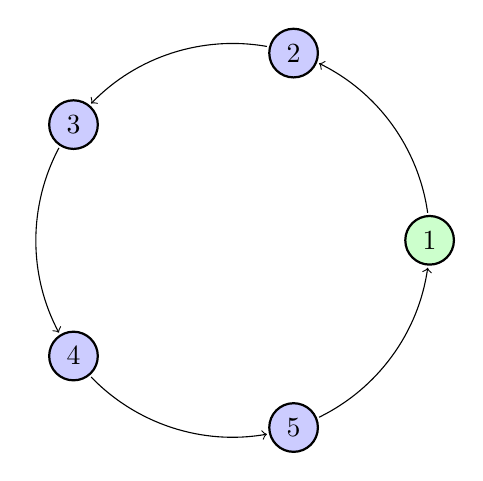
\begin{tikzpicture}[->,
	main node/.style={circle,draw,thick,fill=blue!20,minimum size=4mm},
	leader node/.style={circle,draw,thick,fill=green!20,minimum size=4mm}
]

	\def \n {5};
	\def \r {2.5cm};
	\def \m {8};

	\draw[->] (\m:\r) arc ({\m}:{360/\n -\m}:\r);

	\foreach \s in {2,...,\n} {
		\draw[->] ({360/\n * (\s-1) + \m}:\r) arc ({360/\n * (\s-1) + \m}:{360/\n * (\s) -\m}:\r);
		\node[main node] at ({360/\n * (\s-1)}:\r) {$\s$};
	}
	\node[leader node] at (0:\r) {1};
\end{tikzpicture}
\end{minipage}
\begin{minipage}{.5\textwidth}
\centering
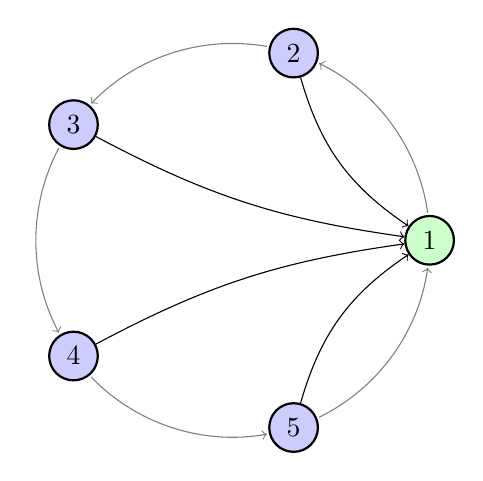
\begin{tikzpicture}[->,
	main node/.style={circle,draw,thick,fill=blue!20,minimum size=4mm},
	leader node/.style={circle,draw,thick,fill=green!20,minimum size=4mm}
]

	\def \n {5};
	\def \r {2.5cm};
	\def \m {8};

	\draw[->,gray] (\m:\r) arc ({\m}:{360/\n -\m}:\r);

	\foreach \s in {2,...,\n} {
		\draw[->,gray] ({360/\n * (\s-1) + \m}:\r) arc ({360/\n * (\s-1) + \m}:{360/\n * (\s) -\m}:\r);
		\node[main node] at ({360/\n * (\s-1)}:\r) (\s) {$\s$};
	}
	\node[leader node] at (0:\r) (L) {1};

	\draw[->] (2) to[bend right=20] (L);
	\draw[->] (3) to[bend right=10] (L);
	\draw[->] (4) to[bend left=10] (L);
	\draw[->] (5) to[bend left=20] (L);
\end{tikzpicture}
\end{minipage}
\end{figure}

\subsubsection{Aggiornamenti allo stato}

\subsubsection{Tolleranza ai guasti}
	Il sistema risulta tollerante ai guasti di tipo crash.
	Nel caso di un guasto di tipo crash sul nodo leader corrente, sara' il
	sistema ad invocare un'eccezione di tipo \textbf{RemoteException} verso
	i nodi interroganti, che lo elimineranno quindi dalla loro lista di
	interrogazione, riconfigurando l'anello.\\
	Nel caso di un guasto di un nodo intermedio il risultato sara' il
	medesimo al momento di un'interrogazione da parte dei vari nodi
	dell'anello.\\
	Questo genere di configurazione mantiene coerente lo stato locale delle
	diverse istanze, poiche' ogni nodo aspetta la risoluzione delle varie
	mosse ad esso precedenti prima di essere interrogato a sua volta e poter
	agire.\\
	Questo schema e' banalmente possibile utilizzando una semplice rete di
	tipo token ring, ma e' stato scelto di implementare il tutto come una
	sorta di cricca per l'aggiornamento automatico e la visualizzazione dei
	risultati con latenze brevi: se si fosse ponderato per una struttura
	completamente circolare (utilizzante lo stesso modello logico) gli
	aggiornamenti allo stato locale sarebbero applicati solamente dopo che
	il controllo (e quindi la leadership) fosse tornata al nodo richiedente,
	risultando in un'attesa pari ad \textbf{N-1} turni; essendo il gioco
	in questione un gioco di logica non propriamente reattivo e con turni
	di gioco potenzialmente molto lunghi e riflessivi e' stato optato
	per un modello piu' pesante da un punto di vista
	di scambio di informazioni che da un punto di vista piu' leggero come
	comunicazioni ma, allo stesso tempo, meno reattivo per tutti i client.
